\documentclass[11pt,a4paper]{article}

\usepackage{graphicx}
\usepackage{listings}
\title{Semaphore using FreeRTOS on LPC2148}


\author{e-Yantra Team}
\date{\today}

\begin{document}
	\maketitle
	\newpage
	\tableofcontents
	\newpage
	\section{Introduction to RTOS}
	\subsection{What is RTOS ?}
	"RTOS" stands for Real-Time Operating System.
	It is a type of operating system used for real time applications in embedded systems.
	RTOS is known for its characteristics that helps is in many applications.
	\begin{itemize}
		
		\item Reliability :\\
		RTOS provides more reliability as compared to GPOS.
		It has more control over events in real time and they are always available to provide service.
		Some systems are required to run for a longer period of time without human intervention, for these purposes RTOS can be very useful.
		
		\item Determinism:\\
		RTOS entirely functions over deadlines which makes            it more efficient.
		It means that for each process a specifc deadline or a time-period is specified within which it has to finish that particular process.
		
		\item Scheduling:\\
		In this operating system, user has more control over scheduling a particular task or a process depending on its priority.
		So we can define the priority for that particular  task and also the frequency with which it should occur ( more like a delay).
		In GPOS all the scheduling functions are process based and user has less control on them.
		Task defined in RTOS are preemptive. 
		Generally, in an operating systems there are two types of tasks viz. High priority tasks and Low priority tasks.
		High priority task can meet their deadlines consistently because of the preemptive property.
		
		\item Scalability:\\
		RTOS is used in wide variety of applications in the field of embedded systems.
		So it is scalable depending on the application requirements (i.e we can add or remove modular components depending on our use).
	\end{itemize}
	
	\subsection{Types of tasks in RTOS}
	\begin{enumerate}
		
		
		\item\textbf{Hard real-time tasks:}\\
		These types of tasks strictly run based on deadlines.
		If a particular task is not finished within the predetermined deadlines  then the system is considered to be a failed system.
		Applications : Anti-missile systems, Air bag mechanisms etc.
		
		\item\textbf{Firm real-time tasks:}\\
		Similar  to hard real-time tasks they should also meet the deadlines.
		But if they don't meet then that doesn't make this a failed system, but the results that are produced after the deadlines are discarded and the utility of the system becomes zero.
		Applications : Multimedia
		
		\item\textbf{Soft real-time systems:}\\
		Here the deadlines are not expressed as some absolute value but they are expressed as a average response time required by the task.
		If the task is finished then the utility of the task is 100%. But if they fail to meet them, then the utility of the system gradually falls depending on the extra time that is taken past the deadline.  
	\end{enumerate}
\newpage	
	\section{What is FreeRTOS}
	
	For statrters FreeRTOS is just a bunch of C files which enables us to implement RTOS in around 32 microcontrollers. FreeRTOS provides files which can be used in multiple microcontrollers with some microcontroller specific support files.
	\\
	\\   
	The main advantage of Implementing FreeRTOS in any microcontroller is the ability to multi-task.
	\\
	\\
	MultiTasking enables the device to execute multiple "Tasks" at the same time.
	MultiTasking in single core systems is implemented by allocating each task a time slice of the processor, In this way Multiple Tasks can be executed at the "same time".
	\\
	\\
	\subsection{Advantage of FreeRTOS}
	\begin{enumerate}
		\item Proper Utilization of Resources.
		\item Low foot-print.
		\item Priority based scheduling of Tasks.
		\item API's for Semaphores.
		\item API's for Making and managing queues.
	\end{enumerate} 

	\subsection{Drawbacks/Disadvantages (write some fancy word)}
	\begin{enumerate}
		\item Use of TaskNotification to implement MailBox.
		\item Not readily Portable to all devices.
		\item Limited source material.
	\end{enumerate} 
\newpage
\section{Requirement}
\begin{enumerate}
	\item Knowledge of C++ 
	\item FreeRTOS source files/API
	\item Keil compiler
	\item Flash magic
	\item FireBird V (LPC2148)
\end{enumerate}


\section{Getting Started !}

	\subsection{DataTypes}
		FreeRTOS defines counterparts of few basic data types
		\\
		\\
\begin{tabular}{|l|l|}
	\hline
	\textbf{Data Type }&\textbf{General Data Type}\\
	 \hline
	 	portCHAR&char\\ \hline
		portSHORT&short\\ \hline
		portLONG&long\\ \hline
		portTickType&This is used to store the tick count\\ \hline
		portBASE\_TYPE&Generally used for Bool type data,is 32 bit for 32 bit type uC\\ \hline
\end{tabular}

	\subsection{Variable Names}
	The Data type is prefixed to the name of a variable for e.g \\
	
	In vTaskDelay "v" denotes the return type "void".\\
	
	In xTaskCreate "x" denotes portBASE\_TYPE.
	
	\subsection{Macros}
	Refer to page 168-169 of the RTOS document by Richard Barry.
	
	\subsection{Creating Tasks}
	
	\begin{lstlisting}
	BaseType_t xTaskCreate(    TaskFunction_t pvTaskCode,
	const char * const pcName,
	unsigned short usStackDepth,
	void *pvParameters,
	UBaseType_t uxPriority,
	TaskHandle_t *pxCreatedTask
	);
	\end{lstlisting}
	
	\begin{itemize}
		\item BaseType\_t :Can be used to check if the task has been created or not.If the returned value is pdTRUE the task has been created if pdFALSE is returned the task was not created.
		
		\item  pvTaskCode:This parameter is a pointer to the task which has been created.
		
		\item pcName :Name given to a Task created so that user can easily identify a task,this parameter enables the programmer to easily identify a task.
		
		\item usStackDepth :The amount of memory/space which a given task is to be allocated is passed as a parameter through this value.
		
		\item uxPriority :Each task is assigned a priority on the basis of which it is allocated the processor time.priority assigned are natural numbers ,as the value of number increases priority increases.
		
		\item pxCreatedTask :Tasks are assigned handles using which they can be referred by other tasks. 
	\end{itemize}
	 
	 Same Task can have multiple instances by varying the priority,parameters passed ,pcName.
	
	\subsection{Frequently used API's}
	\begin{itemize}
		\item vTaskDelay :Takes the Clock Ticks as parameter and suspends the Task for those many cycles. e.g vTaskDelay(1000);
		
		\item vTaskSuspend :Takes Taskhandle as a parameter and Suspends the "passed" task indefinitely.
		e.g. vTaskSuspend(t1) : suspends task t1 
		     vTaskSuspend(NULL) : suspends running task
		
		\item vTaskResume :Also Takes Taskhandle as a parameter resumes the Task from suspended state
		e.g. vTaskResumed(t1) : resumes task t1 
		
		\item tskIDLE\_PRIORITY: Priority of the idle task,used to fix priority of Tasks created.
	\end{itemize}
	\newpage
	
	\section{MultiTasking}
	Multitasking is running multiple processes at the same time.
	In a multi-processor system it implies that each core of processor is executing different tasks i.e. multiple tasks at the same time.
	Whereas in a single processor system the operating system schedules tasks in such a way that all the tasks are performed simultaneously i.e. each task gets a limited amount of Processor time, after the time expires the running task is suspended and another task is executed. The original task gets the resources again when all the tasks are given equal amount of processor time. 
	
	\subsection{Code :}
	\lstinputlisting[language=C]{rtos_multitasking.c}
	
	\subsection{Explanation}
	The given code is used to create 3 tasks 
	\\
	\\
	1st task switches on the buzeer then the task is suspend and after a while the task is resumed and buzzer is switched off.
	\\
	\\
	2nd task is a motion task which aims to give the bot a forward motion.
	\\
	\\
	3rd task prints the value of a counter on the LCD,the value of counter resets when it reaches 100.
	\\
	\\
	The statements for the task which are to be executed are placed inside an infinite loop so that they can be continiously executed.
	\\
	\\
	the xTaskCreate statement "creates tasks" this can be thought of as function call statements which call the respective functions.
	\\ 
	\\
	The vTaskStartScheduler starts scheduling the tasks i.e. allocating processor to the tasks.
	
	If the tasks are not placed in the infinite loop the statements are executed ones and the task is completed.
	
	The ouput can be observed by uploading the code to LPC2148 based FBV.
	  
	  \newpage
	\section{Introduction to semaphore}
	There are a limited number of resources available to any system,Similarly any microcontroller has a limited number  resources available.
	\\ \\
	As the complexity of the application Increases the number of Tasks running also Increases,more and more Tasks compete for the available Processor time or The I/O devices available.
	\\ \\
	To ensure equal availability of resources to all the Tasks Operating Systems provide a facilities through semaphores.
	\\ 
	The Greek word sema means sign or signal, and -phore means carrier . So Semaphore = signalling.
	\\
	Semaphores can be classified into
	\\ 
	\begin{itemize}
	\item Binary Semaphores
	\item Mutex	 
	\item Counting Semaphores
	
	
	\end{itemize}
	\subsection{Binary Semaphores}
	
	Binary semaphores are used for Task synchronisation.
	If a process ocuppies a resource the value of Binary semaphore is 1 else 0 i.e it gives information only if the resource is available or not.
	
	\subsection{Mutex}
	
	Mutex stands for Mutual Exclusion.Any Task which requires a resource can "Block" the resource.when the Task uses the resource it can "Give" the resource.
	
	\subsection{Counting Semaphore}
	
	Counting semaphores are used to count resources and keep track of Multiple resources.
	\\
	 
	\subsection{Mutex vs Binary Semaphore}
	\begin{itemize}
		\item Mutexes are used for Resource Protection from other tasks//processes whereas Binary semaphores are used for task synchronistaion
		\\
		\item It is the responisibility of the occupying function to release the mutex,but a binary semaphore can be released even from ISR or any other functions.
		\\
		\item On the implementation level it is the Responibility of the Coder to ensure that the Mutex is only given by the task which takes it.
		
	\end{itemize}
		
	
	
	
	\newpage	
	\section{Binary Semaphore}
	
\subsection{Code : }
	\lstinputlisting[language=c]{bin.c.}	
	\newpage
\subsection{Explanation}
	\begin{itemize}
	\item \textbf{Variable declaration}	
	
	\begin{lstlisting}
	SemaphoreHandle_t xSemaphore;
	\end{lstlisting}
	
	 This statement declares a variable of type "SemaphoreHandle\_t"
	
	\item \textbf{Creation of the semaphore}
	
	\begin{lstlisting}
	xSemaphore=xSemaphoreCreateBinary( );
	\end{lstlisting}

\item \textbf{Working of code}
	  \\
	  \\
	  The forward function Waits for portMAX\_DELAY i.e for maximum amount of time so that the control of Resources is available.
	  \\
	  \\
	  Similarly the back function waits for maximum time to get access to the resources.
	  \\
	  \\	
	  As soon as execution of Tasks starts the resources are occupied by the back function(vTaskDelay restricts forward function),The control\_switcher function is suspended for 1200 clock counts and Gives away the semaphore.
	  \\
	  \\
	  As soon as the semaphore is released the forward function waiting for allocation of resources occupies them,the cycle continues with control\_switcher releasing the semaphore.  
		\\
		\\
		\\
\item \textbf{Serial monitor Output} 
\\
\\
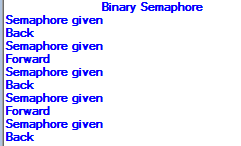
\includegraphics[width=10cm]{bin}

\end{itemize}
\newpage 
\section{Mutex}

\subsection{Code : }
\lstinputlisting[language=c]{mut.c.}	
\newpage

\subsection{Explanation}
\begin{itemize}
	\item \textbf{Variable declaration}	
	
	\begin{lstlisting}
	SemaphoreHandle_t xSemaphore;
	\end{lstlisting}
	
	This statement declares a variable of type "SemaphoreHandle\_t"
	
	\item \textbf{Creation of Mutex}
	
	\begin{lstlisting}
	xSemaphore = xSemaphoreCreateMutex();
	\end{lstlisting}
	
	\item \textbf{Working of code}
	\\
	\\
	There are Two Tasks forward and back, when executed
	\\
	\\
	The forward function Waits for 1000 clock cycles for the resources,In case the resources are not available the Task sends a message about The lack of availability of resources.
		Similarly the back function waits for same amount of time for resources.
	\\
	\\	
	As soon as execution of Tasks starts the resources are occupied by one of the the task and that task blocks the acess of those resources through a mutex.
	\\
	\\
The task executes and when the execution is completed it "Gives" the Mutex and therefore the releases the resources,another waiting task then occupies those resources and blocks for a period of time it requires.
	\\
	\\
	\\
	\item \textbf{Serial monitor Output} 
	\\
	\\
	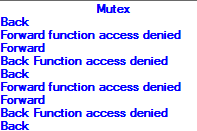
\includegraphics[width=8.5cm]{mut}
\end{itemize}

\newpage 

\section{Counting Semaphore }

\textbf{:Implemented by dining Philosophers Problem}
\subsection{Code : }
\lstinputlisting[language=c]{cont.c.}	
\newpage

\subsection{Explanation}
\begin{itemize}
	\item \textbf{Variable declaration}	
	
	\begin{lstlisting}
	SemaphoreHandle_t xSemaphore;
	\end{lstlisting}
	
	This statement declares a variable of type "SemaphoreHandle\_t"
	
	\item \textbf{Creation of Counting semaphore}
	
	\begin{lstlisting}
xSemaphore = xSemaphoreCreateCounting( 5, 5 );
	\end{lstlisting}
	
	Here 1st parameter gives the maximum count and 2nd parameter is the initial count.
	If the semaphore is used for counting events 2nd parameter would be 0 and if used for resources management it would be equal to maximum or initial count.
	\\
	\item \textbf{Task Creation }
	\begin{lstlisting}
	xTaskCreate(vfork,"Philospher 1", 300 ,"P1",
	 tskIDLE_PRIORITY + 1, NULL);
	.
	.
	\end{lstlisting}
	Here vfork is a single Task which on variation of Parameter P1,P2...etc behaves as a different task,ecah task has its own stack and act as if they are independent.All the tasks have same priority and get equal time at the processor.
	\\
	\item \textbf{Working of code}
	
	The Tasks created are by changing the parameters of a single task.
	\\
	\\
	When each time a "Philosopher" is allocated the processor time it checks for the number of available "Forks".If the forks are available and then check for the Right fork and the philosopher "picks up the left fork" then when the "Philosopher" again gains the processor time it waits for Left fork to be available and proceeds to eat.
	
	when 5 "Philosophers" are allocated simulatenously the semaphore keeps track of the available forks .
	
	
	\newpage
	\item \textbf{Serial monitor output}
	\\
	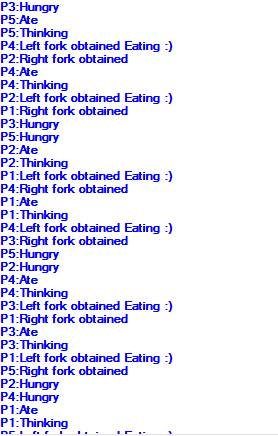
\includegraphics[width=12cm]{cont}
\end{itemize}
\newpage


\section{Task Notification}
	There occurs instances when tasks needs to communicate with each other.Semaphores are one of the methods by which tasks communicate with each other.Two other methods by which tasks communicate with each other are 
	\begin{enumerate}
		\item MailBox
		\item Queues
	\end{enumerate}
	
   Tasks in mailbox communicate by sending "Mails" to each other.In FreeRTOS mailbox is implemented by Task Notification.
   
   Each Task has an associated notification value using which they can be "notified".When a task is notified, Task notifications can update the receiving task's notification value in the following ways:
   \begin{itemize}
   	 
\item Set the receiving task's notification value without overwriting a previous value
\item Overwrite the receiving task's notification value
\item Set one or more bits in the receiving task's notification value
\item Increment the receiving task's notification value 
   
   \end{itemize}
   \newpage
   \subsection{Code:}
   \lstinputlisting[language=c]{mbox.c.}	
   \newpage
   
   \subsection{Explanation}
   
   Above is a simple code which has four tasks(vn1,vn2,vn3,vn4) which notify a 5th task 'noticier',The 5th task prints which task notified it. 
   \\
   \\
   \begin{itemize}
   	\item \textbf{xTaskNotify()}
   	This function is used to notify other tasks general format is as specified below 
   		\begin{lstlisting}
   		xTaskNotify(xHandle, 0x03, eSetBits);
   		\\(Task Handle,Notification value,eAction)
   		\end{lstlisting}
  
  
   	\textbf{Parameters}
   	\begin{itemize}
   		\item \textbf{Task handle}:The handle of the task which needs to be notified.
   		\item \textbf{Notification value}:Value used for notification
   		\item \textbf{eAction}:The type of action which is to be carried out upon the specified task.The types are as specified below:
		   		\begin{itemize}
		   			\item eNoAction :The Task receives the value but no action takes place,can used to Resume a suspened task.
		   			
		   			\item eSetBits :The existing Notification value will be Bitwise OR-ed with the Notified value to obtain a new value.
		   			
		   			\item eIncrement :Increments the existing value.
		   			
		   			\item eSetValueWithOverwrite :Overwrites the existing Notification value.
		   			
		   			%\item eSetValueWithoutOverwrite :Didn't understand this part
		   			
		   		\end{itemize}
		   		
   	\end{itemize}
   	
   	\textbf{Return value :}
   	  	Returns pdTRUE if Task has been Notified else pdFALSE.
   	
   	\item \textbf{xTaskNotifyWait() } The Function waits to receive a Notification and has parameters which govern the actions upon the received data.
   	\begin{lstlisting}
   	xTaskNotifyWait( 0x00,0xffff,&ulNotifiedValue,1000 )
   	\\(clear bits on entry,clear bits on exit,notified value,time out)
   	\end{lstlisting}
   	\textbf{Parameters}
   	\begin{itemize}
   		\item \textbf{ulBitsToClearOnEntry}:Specifies the Bit position which needs to be cleared as soon as the Notification is received.
   	    
   	    \item \textbf{ulBitsToClearOnExit }:Specifies the Bit position which needs to be cleared before xTaskNotifyWait() function exits if a notification was received
   	    
   	    \item \textbf{pulNotificationValue}:The Notification value before exit is taken and stored in this.
   	       
   	    \item \textbf{xTicksToWait  } :This specifies the timeout period for which the function call waits for a notification.
   \end{itemize}
   
   \item \textbf{Working}
   \newline
   Tasks vn1,vn2,vn3,vn4 With different frequencies send a "message" to a noticer task through a hex value,these hex values are compared to find out which task sent the message.
   \\
   For the first few ticks no task is sending a notification so the noticier prints a "No Notice" message,as It starts receiving messsages it starts acknowledging the received messages. 
   \end{itemize}
   
   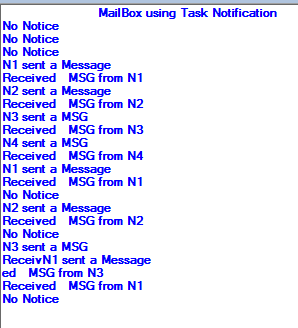
\includegraphics[width=12cm]{mbox}
	\newpage
	\section{Queue}
	 \subsection{Intro}
	 In RTOS, inter-process communication is possible. It means that you can communicate between two task and control them on the basis of this communication.\\ But first we need to understand \textbf {what is queue?}\\
	Consider a dynamic buffer. Dynamic in the sense of memory allocation. We can allocate the size of the buffer as per our requirements. There are two things that we can change, one is the size of each data the buffer can carry and other is the number of data the buffer can send with each data of the size defined by us. this buffer is known as queue.\\
	
	\subsection{Code}
	\lstinputlisting[language=c]{q.c.}
	
	\subsection{Explanation}
	\begin{itemize}
		\item \textbf{QueueHandle\_t} :A predefined data type used to reference a queue.
		
		\begin{lstlisting}
		QueueHandle_t xQueue= 0;
		\end{lstlisting}	
		
		\item \textbf{xQueueCreate(a,b)}:Creates a queue of 'a' continuous memory locations,where each memory location is of 'b' bytes each.It returns a 'pointer' to the queue which is stored in the queuehandle.
		
		\begin{lstlisting}
		xQueue = xQueueCreate(7,40);
		\end{lstlisting}
		
		\item \textbf{xQueueSend(QueueHandle,data,timeout period)}:This function is used to send data to queue,It has three parameters
		
		\begin{enumerate}
			\item\textbf{QueueHandle}:It gives the address of the queue in which data has to be stored.
			
			\item\textbf{Data}:The data which needs to be stored in the queue.
			
			\item\textbf{Timeout period}:This specifies the amount of time for which the function waits if the queue is unavailable(i.e data is being sent to queue or queue is full) 
			\newline		
		\end{enumerate}
		
		\textbf{Return value :}Returns pdTRUE if Data has been sent to Queue else pdFALSE e.g..
		\begin{lstlisting}
		if(xQueueSend(xQueue,p,1000) == pdTRUE)
		...
		\end{lstlisting}
	\item \textbf{xQueueReceive(QueueHandle,data,timeout period):}This function is used to receive data from a queue,It has three parameters
	
	\begin{enumerate}
		\item\textbf{QueueHandle}:It gives the address of the queue from which data has to be obtained.
		
		\item\textbf{Data}:A variable in which the poped data has to be stored.
		
		\item\textbf{Timeout period}:This specifies the maximum amount of time for which the function waits if the queue is unavailable(i.e data is being received by another task or queue is empty) 
		\newline		
	\end{enumerate}
	\textbf{Return value :}Returns pdTRUE if Data has been Received from the Queue, pdFALSE id queue is empty e.g..
	\begin{lstlisting}
	if(xQueueReceive(xQueue,rx,1000) == pdTRUE)
	...
	\end{lstlisting}
	
	\item\textbf{Working of code:}
	Initially a queue is created which can accomodate 7 elements in which each of them can occupy 40 Bytes.
	
	There are 4 tasks which send data to the queue and one task which receives data from the queue.
	
	As the tasks are created data is pushed into the queue and the receiving task is resumed which inturn pops the data and prints them through the serial comm port.
	
	From the Output screenshots it can be observed how  data pushed 1st is popped out 1st (Queue mechanism).  
	\end{itemize}
	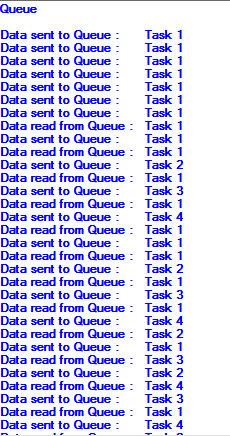
\includegraphics[width=12cm]{q}
	\section{Application Based Experiments}
	\subsection{State collection}
	State collection involves storing data of sensors at each instance.The advantage of having the state of robot(i.e sensor values) is that it would help in debugging or simulating an already conducted experiment.
	
	The experiment given below would collect sensor data,store it in a string and send it via serial port every 100ms and there is a corresponding python script which would store the collected data with the time stamp in a script file.
	\\
	Each sensor data is seperated by a ',' and each set of data is seperated by delemiters ',00,255,'
	\subsubsection{State collection Code}
	\lstinputlisting[language=c]{statecol.c.}
	\newpage 
	\subsubsection{Python script}
	\lstinputlisting[language=python]{serialcomm.py.}
	
	\subsection{Sample output}
	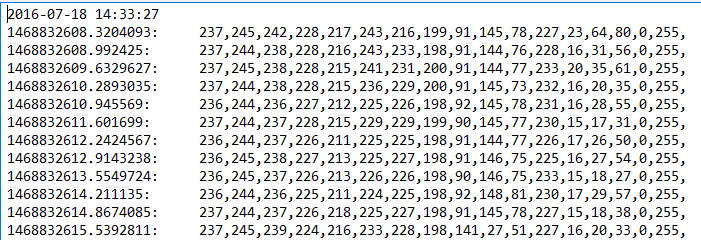
\includegraphics[width=14cm]{serialcomm}
	
	\newpage
	\section{References}
	\begin{enumerate}
	\item  http://www.rtos.be/2013/05/mutexes-and-semaphores-two-concepts-for-two-different-use-cases/
	
	\item http://www.ocfreaks.com/cat/embedded/lpc2148-tutorials/
	\item http://www.freertos.org/Inter-Task-Communication.html
	\item http://tinymicros.com/
	\item http://www.profdong.com/elc4438\_spring2016/\\USINGTHEFREERTOSREALTIMEKERNEL.pdf
	\end{enumerate}	
	\end{document}


